
\lecture{20}{Free Energy and Chemical Equilibrium}{Qiang Zhu}{scribe-name1,2,3}

\section{Gibbs Free Energy and Chemical Potential}

\begin{equation}\mu  = (\frac{\partial {G}}{\partial {N}})_{T,P} \end{equation}
\begin{equation}\mu  = (\frac{\partial {F}}{\partial {N}})_{T,V} \end{equation}

We can derive the relation between $\mu$ and $G(F)$ as follows.
\begin{equation} G = N\mu \end{equation}
or 
\begin{equation} F = N\mu \end{equation}

\begin{enumerate}
\item extensive quantities: $V, N, S, U, H, F, G, M$
\item intensive quantities: $T, P, \mu, \rho$
\end{enumerate}

When the total amount doubles, the values of extensive quantities will double as well. 
When you try to sum up along $-(\frac{\partial {F}}{\partial {N}})_{T,V}$, it would fail.
But it works for $G$, thus we have 

\begin{equation}G  = N_1\mu_1 + N_2\mu_2 + .... = \sum_i N_i\mu_i \end{equation}

Let's try to use this formula to calculate $\mu$. 
\begin{equation}\frac{\partial \mu}{\partial P} = \frac{1}{N} \frac{\partial G} {\partial P} = \frac{V}{N} = \frac{kT}{P} ~~~~\text{ideal gas}\end{equation}
\begin{equation} \mu(T,P) - \mu(T,P0) = kT \text{ln}(P/P0) \end{equation}
This tells you how $\mu$ varies as the pressure changes.

\section{Chemical Equilibrium}
An interesting fact about chemical reactions is that they hardly even go to completion. Consider the dissociation of water into
H$^+$ and OH$^-$ ions,
\ce {H2O <-> H$^+$ + OH$^-$} \\
This reaction tends to strongly go to the left. But it won't be the whole story. Otherwise, there would be no ions in a glass of water!

How do we understand this? At room temperature, the water molecules are constantly colliding with each other at rather high speed. Every once in a while, one of these collisions is violent enough to break a molecule apart into two ions. The ions then tend to separate. Eventually an equilibrium is reached between the breaking apart and recombining.

This phenomenon could also be explained by the Gibbs free energy as a function of the balance between products and reactants. If we draw $G$ as a function of the extent of the reaction, just like we did with the phase transitions, the reaction could be considered as the mixing between reactants and products. Without mixing, $G-x$ should behave like a linear curve, where $G$ reaches minimum and maximum at $x$=0 or 1. With mixing, the energy might reach a minimum at some state between 0 and 1.

\begin{figure}[h]
\centering
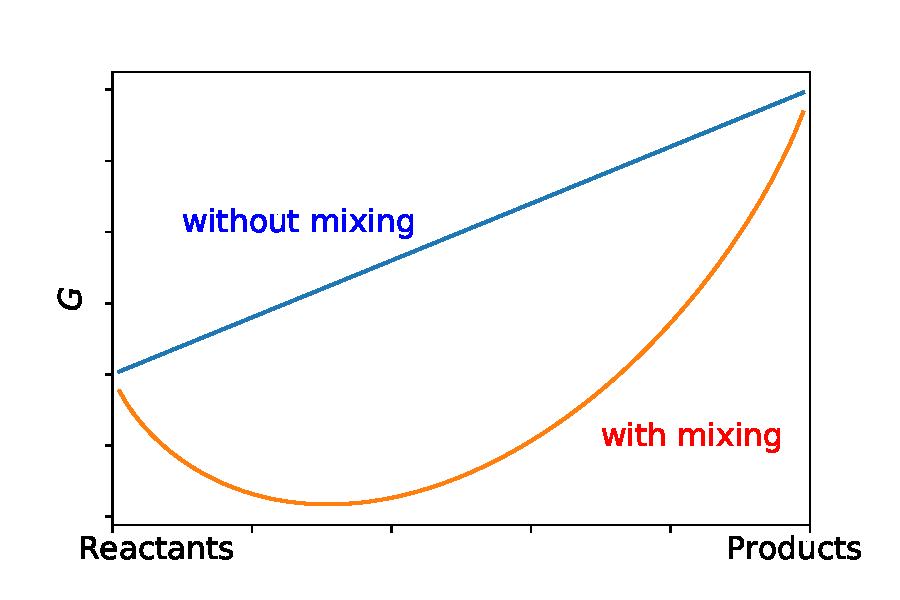
\includegraphics[width=10cm]{imgs/Reaction.pdf}
\caption{The free energy plot as a function of the extent of the chemical reaction. }
\end{figure}


We can characterize the equilibrium point by the condition that the slope of $G$ is zero. Therefore,
\begin{equation} 
0 = dG = \sum_i \mu_i dN_i
\end{equation} 

This actually tells us the chemical potentials must be satisfied at equilibrium.

{\bf exercise} Write down the equilibrium condition for each of the following reactions.
\begin{enumerate}
\item \ce {2H <-> H2}
\item \ce {N2 + 3H2 <-> 2NH3}
\item \ce {2CO + O2 <-> 2CO2}
\item \ce {CH4 + 2O2 <-> 2H2O + CO2}
\end{enumerate}

\section{Nitrogen Fixation}
Let's investigate a reaction in more detail. The reaction that N$_2$ and H$_2$ combine to form ammonia is called nitrogen fixation
because it puts the nitrogen into a form that can be used by plants to synthesize amino acids and other important molecules.
Under the equilibrium condition, the chemical potentials must satisfy the following,
\begin{equation}
\mu^0(N_2) + kT\text{ln}\frac{P(N_2)}{P^0} + 3\mu^0(H2) + 3kT\text{ln}\frac{P(H_2)}{P^0}  =  2\mu^0(NH_3) + 2kT\text{ln}\frac{P(NH_3)}{P^0}.
\end{equation}

Normally, we take $P^0$ to be 1 bar. Gathering all the $\mu^0$, we come to,
\begin{equation}
kT\text{ln}\frac{P(N_2)}{P^0} + 3kT\text{ln}\frac{P(H_2)}{P^0} - 2kT\text{ln}\frac{P(NH_3)}{P^0} = 
2\mu^0({NH_3}) - \mu^0(N_2) - 3\mu^0({H_2})
\end{equation}

\begin{equation}
RT\text{ln}\frac{P(N_2)P^3(H_2)}{P^2(NH_3)(P^0)^2} = \Delta{G^0}
\end{equation}
or
\begin{equation}
\frac{P(N_2)P^3(H_2)}{P^2(NH_3)(P^0)^2} = e^{\Delta{G^0}/RT}
\end{equation}

Here we define the right side as the equilibrium constant, $K$.

\section{van't Hoff equation}
What's the temperature dependence of $K$?
\begin{equation}
\frac{d\text{ln}K}{dT} = \frac{d(-\Delta{G^0}/RT)}{dT} =  \frac{d(-\Delta{H^0-TS}/RT)}{dT} = \frac{\Delta{H^0}}{RT^2}.
\end{equation}
If $\Delta{H^0}$ is positive, then higher temperatures are needed to make the reaction tend more to the right.

A catalyst only changes the rate (kinetics) 
$P$, $T$ help to improve $K$

\section{Homework}
Problem: 5.84, 5.85


